%%%%%%%%%%%%%%%%%%%%%%%%%%%%%%%%%%%%%%%%%%%%%%%%%%%%%%%%%%%
% --------------------------------------------------------
% Rho
% LaTeX Template
% Version 2.1.1 (01/09/2024)
%
% Authors: 
% Guillermo Jimenez (memo.notess1@gmail.com)
% Eduardo Gracidas (eduardo.gracidas29@gmail.com)
% 
% License:
% Creative Commons CC BY 4.0
% --------------------------------------------------------
%%%%%%%%%%%%%%%%%%%%%%%%%%%%%%%%%%%%%%%%%%%%%%%%%%%%%%%%%%%

\documentclass[9pt,letterpaper,onecolumn]{rho-class/rho}
\usepackage[spanish,es-nodecimaldot,es-noindentfirst]{babel}
\usepackage{amsmath}
\usepackage{graphicx}
\usepackage{hyperref}

\setbool{rho-abstract}{true}
\setbool{corres-info}{true}

%----------------------------------------------------------
% TITLE
%----------------------------------------------------------

\title{}

%----------------------------------------------------------
% AUTHORS AND AFFILIATIONS
%----------------------------------------------------------

\author[$\dagger$]{Diego Sanhueza}
\author[$\dagger$]{Manuel González}
\author[$\dagger$]{Claudio Matulich}

%----------------------------------------------------------

\affil[$\dagger$]{Universidad de Magallanes}

%----------------------------------------------------------
% DATES
%----------------------------------------------------------

\dates{\today}

%----------------------------------------------------------
% FOOTER INFORMATION
%----------------------------------------------------------

\title{Diseño de Algoritmos - PR3: Algoritmos de Búsqueda de Patrones en Documentos}

%----------------------------------------------------------
% ARTICLE INFORMATION
%----------------------------------------------------------

%----------------------------------------------------------
% ABSTRACT
%----------------------------------------------------------

\begin{abstract}
%Resumen del informe
En este informe se presenta el desarrollo de un sistema de búsqueda de patrones en documentos, implementando algoritmos avanzados y estructuras de datos eficientes. El objetivo es analizar el rendimiento de estos algoritmos en términos de tiempo de ejecución, número de comparaciones y accesos a memoria, utilizando un conjunto de documentos preprocesados. Se implementaron varios algoritmos de búsqueda, incluyendo KMP y Boyer-Moore, y se desarrollaron estructuras de datos para indexación y recuperación de información. Además, se aplicaron técnicas de preprocesamiento de texto para mejorar la eficiencia y precisión de las búsquedas.
\end{abstract}

%----------------------------------------------------------

\begin{document}
\maketitle
\thispagestyle{firststyle}
\tableofcontents

\section{Introducción}

La gestión y recuperación de información textual es un área fundamental dentro de la informática, con aplicaciones que van desde motores de búsqueda a nivel web hasta herramientas de análisis documental en entornos locales. Este proyecto se enmarca en dicho contexto, proponiendo el desarrollo de un sistema de búsqueda textual capaz de analizar, procesar y extraer información relevante desde documentos en formatos \texttt{.txt} y \texttt{.html}.

El sistema ha sido implementado completamente en lenguaje C (estándar C11), priorizando el uso de estructuras de datos básicas y técnicas algorítmicas eficientes. Esto permite no solo evaluar el desempeño práctico del motor, sino también profundizar en el entendimiento de cómo operan internamente los algoritmos clásicos de búsqueda de patrones y estructuras como tablas hash e índices invertidos.

El motor implementado cuenta con módulos de:
\begin{itemize}
    \item Preprocesamiento de texto, incluyendo limpieza de etiquetas HTML y normalización de caracteres,
    \item Filtrado de palabras irrelevantes (stopwords),
    \item Construcción de índices para facilitar la localización de palabras,
    \item Búsqueda de patrones mediante algoritmos como Boyer-Moore, Knuth-Morris-Pratt y Shift-And,
    \item Detección de similitud entre documentos,
    \item Identificación de palabras clave frecuentes, y
    \item Generación de rankings de relevancia según una consulta dada.
\end{itemize}

A lo largo del informe se describirá en detalle el funcionamiento interno del sistema, las decisiones de diseño adoptadas, y se analizarán cuantitativamente los resultados obtenidos mediante distintas métricas, como tiempo de ejecución, comparaciones realizadas y accesos a memoria. La modularidad del sistema y su enfoque didáctico lo convierten en una herramienta útil tanto para el aprendizaje como para la experimentación con algoritmos de búsqueda y procesamiento de texto.


\section{Objetivos}
\begin{itemize}
    \item Implementar algoritmos avanzados de búsqueda de patrones en texto.
    \item Desarrollar estructuras de datos eficientes para indexación y recuperación de información.
    \item Analizar empíricamente la complejidad y rendimiento de los algoritmos.
    \item Aplicar los algoritmos a un problema práctico de procesamiento de documentos.
    \item Implementar técnicas de preprocesamiento de texto para mejorar la eficiencia de búsqueda.
    \item Documentar adecuadamente el código y los resultados del análisis.
\end{itemize}

\section{Fundamento teórico}
\label{sec:fundamentoteorico}

Este proyecto se apoya en conceptos fundamentales de algoritmos de búsqueda de patrones, estructuras de datos para indexación, y métricas de similitud textual. A continuación se presenta un resumen de las bases teóricas empleadas.

\subsection{Algoritmos de búsqueda de patrones}

La localización de una subcadena dentro de un texto es una operación central en motores de búsqueda. En este proyecto se implementaron tres algoritmos clásicos:

\subsubsection*{Knuth–Morris–Pratt (KMP)}

El algoritmo KMP permite buscar una cadena patrón dentro de un texto con una complejidad temporal de $\mathcal{O}(n + m)$, donde $n$ es la longitud del texto y $m$ la del patrón. Utiliza un arreglo auxiliar (LPS, \textit{longest proper prefix which is also suffix}) para evitar comparaciones redundantes cuando ocurre una desalineación, mejorando el rendimiento en patrones repetitivos.

\subsubsection*{Boyer–Moore (Heurística del mal carácter)}

Boyer–Moore es uno de los algoritmos más eficientes en la práctica para textos largos, ya que compara el patrón desde el final hacia el principio. En este trabajo se utiliza la heurística del \textit{mal carácter}, que permite saltar varias posiciones del texto si se detecta una incompatibilidad temprana, basándose en la última ocurrencia del carácter en el patrón. Su complejidad es en el peor caso $\mathcal{O}(n \cdot m)$, pero típicamente mucho menor.

\subsubsection*{Shift–And}

Este algoritmo está basado en operaciones bit a bit y es eficiente para patrones cortos (máximo 31 caracteres en este proyecto). Representa el patrón mediante máscaras binarias y actualiza un registro (\texttt{R}) que permite detectar coincidencias completas en tiempo constante por carácter, resultando en una complejidad lineal $\mathcal{O}(n)$.

\subsection{Estructuras de datos auxiliares}

\subsubsection*{Tabla hash}

Para gestionar la frecuencia de palabras y calcular similitudes, se utiliza una tabla hash con encadenamiento por listas enlazadas. Esta estructura permite almacenar palabras únicas junto a su frecuencia de aparición, y acceder a ellas en tiempo promedio $\mathcal{O}(1)$.

\subsubsection*{Índice invertido}

Un índice invertido asocia cada palabra del vocabulario con las posiciones donde aparece en el texto. Esta técnica, ampliamente utilizada en sistemas de recuperación de información, permite búsquedas más rápidas al evitar recorrer todo el texto en cada consulta. En este proyecto, el índice puede guardarse en disco y ser reutilizado posteriormente.

\subsection{Similitud y distancia}

\subsubsection*{Similitud de Jaccard}

Para comparar el contenido de dos documentos, se emplea la métrica de Jaccard, definida como la razón entre el número de elementos comunes y el total de elementos distintos. En este caso, los elementos son las palabras únicas de cada texto. Se implementa mediante una tabla hash compartida entre ambos documentos.

\subsubsection*{Distancia de Levenshtein}

Esta distancia mide el número mínimo de operaciones (inserción, eliminación o sustitución) necesarias para transformar una palabra en otra. Es útil para detectar errores tipográficos o variaciones cercanas en las consultas. La complejidad es $\mathcal{O}(n \cdot m)$ para palabras de longitud $n$ y $m$.

\subsection{Eliminación de \textit{stopwords}}

Las \textit{stopwords} son palabras de alta frecuencia y bajo valor semántico (e.g., "el", "de", "y"), que suelen eliminarse para mejorar la precisión en tareas de búsqueda y análisis. En este sistema, se utiliza un listado en español que se filtra antes de construir índices o calcular frecuencias.

\vspace{0.5em}
Este conjunto de herramientas teóricas y algorítmicas sienta las bases para el diseño e implementación del sistema propuesto, cuya arquitectura modular y análisis de rendimiento se presentan en las siguientes secciones.


\section{Descripción del proyecto}
\label{sec:implementacion}

El sistema desarrollado es un motor de búsqueda textual modular y extensible, implementado íntegramente en lenguaje C, que permite realizar búsquedas eficientes, analizar documentos, calcular métricas de similitud y construir índices persistentes.

\subsection{Estructura general}

El proyecto se organiza en varios módulos contenidos en las carpetas \texttt{src/} y \texttt{incs/}, con el archivo \texttt{main.c} como punto de entrada. Se emplea un sistema de compilación vía \texttt{Makefile} y el programa puede ejecutarse mediante un script de automatización \texttt{run.sh}.

La funcionalidad del sistema se divide en las siguientes etapas:

\begin{enumerate}
  \item \textbf{Carga y normalización de texto}: se eliminan etiquetas HTML y se normalizan caracteres, incluyendo acentos y mayúsculas.
  \item \textbf{Filtrado de palabras irrelevantes (stopwords)}: se eliminan palabras comunes que no aportan significado semántico relevante.
  \item \textbf{Construcción de índices}: se crean estructuras auxiliares (tabla hash e índice invertido) para acelerar búsquedas futuras.
  \item \textbf{Ejecución de búsqueda}: se permite al usuario seleccionar entre diferentes algoritmos de búsqueda por patrones.
  \item \textbf{Análisis y visualización}: se recopilan métricas de rendimiento y se generan salidas interpretables por el usuario.
\end{enumerate}

\subsection{Interfaz de uso}

El sistema se ejecuta desde línea de comandos, permitiendo una variedad de combinaciones de opciones. Por ejemplo:

\begin{itemize}
  \item \texttt{./run.sh -f archivo.txt --bm --pattern "palabra"} \hfill (búsqueda Boyer-Moore)
  \item \texttt{./run.sh --compare doc1.txt doc2.txt} \hfill (similitud entre documentos)
  \item \texttt{./run.sh -f archivo.txt --detect} \hfill (palabras clave del texto)
  \item \texttt{./run.sh -f archivo.txt --proximity "term" --tolerance 2} \hfill (palabras similares)
  \item \texttt{./run.sh --ranking "palabra"} \hfill (ranking de documentos)
\end{itemize}

\subsection{Principales funcionalidades implementadas}

\begin{description}
  \item[Búsqueda de patrones:] el usuario puede buscar una palabra o patrón utilizando KMP, Boyer-Moore o Shift-And, especificando el archivo de entrada.
  
  \item[Similitud de documentos:] se calcula el índice de Jaccard entre dos archivos de texto, reportando un porcentaje de similitud.
  
  \item[Palabras similares:] usando la distancia de Levenshtein, el sistema encuentra términos cercanos a una consulta dada, dentro del mismo texto.
  
  \item[Índice invertido persistente:] se construye una estructura que asocia palabras con sus posiciones y puede guardarse y cargarse desde disco para evitar reprocesamiento.
  
  \item[Ranking de documentos:] al buscar una palabra, se muestra una tabla con los documentos donde aparece, ordenados por número de ocurrencias.
  
  \item[Visualización de métricas:] para cada búsqueda se registran comparaciones, accesos a memoria y tiempo de ejecución en archivos CSV que luego pueden graficarse.
\end{description}

\subsection{Modularidad del código}

Cada funcionalidad está implementada en módulos separados:
\begin{itemize}
  \item \texttt{load.c}, \texttt{stopwords.c} y \texttt{tokenizer.c} para carga, limpieza y segmentación del texto.
  \item \texttt{boyer\_moore.c}, \texttt{kmp.c}, \texttt{shift\_and.c} para los algoritmos de búsqueda.
  \item \texttt{hash.c}, \texttt{inverted\_index.c} para estructuras auxiliares.
  \item \texttt{calculate\_similarity.c}, \texttt{levenshtein.c}, \texttt{ranking.c} para análisis textual.
  \item \texttt{main.c} como punto de integración de todas las opciones.
\end{itemize}

Esta arquitectura modular permite aislar responsabilidades, facilitar pruebas independientes y extender el sistema con nuevos algoritmos o estructuras de manera sencilla.


\section{Requisitos Técnicos}
Como requisitos técnicos, el sistema debe ser capaz de manejar archivos de texto y HTML, realizar búsquedas exactas y aproximadas, y proporcionar estadísticas sobre los documentos procesados. Además, debe contar con una interfaz de línea de comandos para facilitar su uso.


\section{Diseño del Sistema}
\label{sec:diseno}

El sistema desarrollado está organizado en módulos claramente definidos que permiten cargar, procesar, indexar y buscar información dentro de documentos de texto plano o en formato HTML. Su arquitectura fue concebida con un enfoque modular, lo que facilita tanto el mantenimiento como la extensión de nuevas funcionalidades.

\subsection{Arquitectura del Sistema}
Descripción general de la arquitectura del sistema, incluyendo módulos principales y su interacción.

El núcleo del sistema se estructura en torno a cinco componentes principales: preprocesamiento, indexación, búsqueda, análisis y la interfaz de usuario. Estos módulos interactúan entre sí mediante funciones bien delimitadas, lo que permite separar la lógica de negocio de la entrada/salida y facilita pruebas unitarias.

\subsection{Módulos Principales}
\begin{itemize}
    \item \textbf{Carga y Preprocesamiento de Documentos:}  
    Módulo encargado de leer los archivos, extraer texto y metadatos, y aplicar técnicas de preprocesamiento. Incluye limpieza de etiquetas HTML, normalización de caracteres, y tokenización. Se implementa en \texttt{load.c}, \texttt{stopwords.c} y \texttt{tokenizer.c}.

    \item \textbf{Indexación de Documentos:}  
    Módulo que construye y actualiza índices para facilitar búsquedas rápidas. Se utilizan dos estructuras: una tabla hash para frecuencias de palabras y un índice invertido persistente que asocia cada término con sus posiciones en el texto.

    \item \textbf{Motor de Búsqueda:}  
    Implementa los algoritmos de búsqueda de patrones y maneja las consultas del usuario. Permite elegir entre KMP, Boyer-Moore y Shift-And, cada uno con sus propias características de eficiencia y uso.

    \item \textbf{Análisis de Texto:}  
    Proporciona estadísticas sobre los documentos, como palabras clave, similitud entre textos y detección de términos cercanos usando la distancia de Levenshtein. También se incluye una funcionalidad de ranking de documentos según la relevancia de un término.

    \item \textbf{Interfaz de Línea de Comandos:}  
    Permite a los usuarios interactuar con el sistema a través de comandos específicos. El archivo \texttt{main.c} interpreta los argumentos y redirige la ejecución al módulo correspondiente.
\end{itemize}

\subsection{Algoritmos de Búsqueda de Patrones}
% Descripción de los algoritmos implementados (KMP, Boyer-Moore, Shift-And, etc.), detalles de implementación y optimizaciones.

En este proyecto se implementaron tres algoritmos principales para la búsqueda de patrones en texto:

\begin{itemize}
    \item \textbf{KMP (Knuth-Morris-Pratt):}  
    Utiliza un arreglo de prefijos (LPS) para evitar comparaciones redundantes y mejorar la eficiencia al buscar patrones. Se registran comparaciones, accesos a memoria y tiempo de ejecución, guardando los resultados en CSV para su análisis.

    \item \textbf{Boyer-Moore (mal carácter):}  
    Implementado usando la heurística del mal carácter, permite saltos eficientes en el texto y reduce el número de comparaciones. También mide el rendimiento y almacena los resultados en un archivo CSV.

    \item \textbf{Shift-And:}  
    Algoritmo basado en operaciones a nivel de bits, eficiente para patrones cortos (hasta 31 caracteres). Utiliza máscaras de bits para representar el estado de coincidencia y también registra métricas de rendimiento.
\end{itemize}

% Recomendación: Aquí se puede incluir una tabla comparativa de resultados experimentales entre los algoritmos, o un gráfico de barras mostrando el tiempo de ejecución y comparaciones.

% kmp
% El algoritmo KMP utiliza un arreglo de prefijos (LPS) para evitar comparaciones redundantes al buscar patrones. También se registran comparaciones, accesos a memoria y tiempo de ejecución, guardando los resultados en CSV para su análisis.

% boyer-moore
% El algoritmo de Boyer-Moore fue implementado utilizando la heurística del mal carácter. Esta técnica permite buscar un patrón dentro de un texto de manera eficiente, realizando comparaciones de derecha a izquierda y utilizando una tabla de desplazamientos para saltar posiciones cuando ocurre una discrepancia.  
% La implementación cuenta el número de comparaciones, accesos a memoria y mide el tiempo de ejecución, almacenando estos resultados en un archivo CSV para su posterior análisis y comparación con otros algoritmos.

\subsection{Estructuras de Datos para Indexación}
% Explicación de las estructuras usadas (Trie, índice invertido, tabla hash, filtro de Bloom, etc.).

Para facilitar búsquedas rápidas y eficientes, se utilizaron principalmente dos estructuras:

\begin{itemize}
    \item \textbf{Índice invertido:}  
    Permite asociar cada palabra con las posiciones donde aparece en los documentos, facilitando búsquedas exactas y consultas booleanas. El índice puede persistirse en disco para ser reutilizado en futuras ejecuciones.

    \item \textbf{Tabla hash:}  
    Usada para calcular la frecuencia de palabras y detectar palabras clave en los textos. También se emplea para implementar la métrica de similitud de Jaccard en la comparación entre documentos.
\end{itemize}

% Recomendación: Se puede agregar un ejemplo de cómo se almacena una palabra y sus posiciones en el índice invertido.

\subsection{Técnicas de Preprocesamiento de Texto}
% Descripción de las técnicas aplicadas (tokenización, normalización, stopwords, stemming, etc.).

El preprocesamiento es fundamental para mejorar la calidad de las búsquedas. Se aplicaron las siguientes técnicas:

\begin{itemize}
    \item \textbf{Tokenización:}  
    Separación del texto en palabras o tokens, ignorando puntuación y delimitadores no alfabéticos.

    \item \textbf{Normalización:}  
    Conversión a minúsculas y eliminación de acentos/caracteres especiales para evitar variaciones innecesarias en las búsquedas.

    \item \textbf{Eliminación de stopwords:}  
    Se eliminan palabras comunes que no aportan significado relevante (como "el", "la", "de", etc.) a través de un archivo externo de lista de términos.
\end{itemize}

% Recomendación: Se puede mostrar un ejemplo de texto antes y después del preprocesamiento.

\subsection{Framework de Análisis de Rendimiento}
% Cómo se midió el rendimiento, qué métricas se usaron y cómo se generaron los datos de prueba.

Para evaluar los algoritmos, se midieron las siguientes métricas en cada búsqueda:

\begin{itemize}
    \item \textbf{Comparaciones:}  
    Número de comparaciones realizadas entre caracteres del texto y del patrón.

    \item \textbf{Accesos a memoria:}  
    Cantidad de veces que se accede a posiciones de texto o patrones, representando el costo de lectura.

    \item \textbf{Tiempo de ejecución:}  
    Medido en milisegundos usando funciones del sistema como \texttt{clock()} para tener referencia temporal del desempeño.
\end{itemize}

Los resultados se almacenan en archivos CSV para facilitar su análisis y comparación. Se usaron textos de prueba de diferentes tamaños y patrones variados.

% Recomendación: Aquí se puede incluir un gráfico de líneas mostrando la evolución del tiempo de ejecución según el tamaño del texto o patrón.


\section{Desarrollo del Sistema}

\subsection{Carga y Preprocesamiento de Documentos}
%Soporte para archivos de texto y HTML, extracción de texto y metadatos.

El sistema permite cargar archivos en formato \texttt{.txt} o \texttt{.html}, manejando ambos de forma transparente. En el caso de archivos HTML, se realiza un proceso de limpieza que remueve todas las etiquetas y conserva únicamente el contenido textual. Una vez extraído el texto, se aplica una etapa de preprocesamiento que consiste en:

\begin{itemize}
    \item \textbf{Normalización:} convierte el texto a minúsculas y reemplaza caracteres acentuados por sus equivalentes sin tilde.
    \item \textbf{Tokenización:} divide el texto en palabras utilizando separadores como espacios, signos de puntuación y saltos de línea.
    \item \textbf{Eliminación de stopwords:} filtra palabras de alto uso y bajo contenido semántico (por ejemplo, “el”, “de”, “y”) utilizando una lista personalizada.
\end{itemize}

Estas técnicas permiten reducir el ruido en las búsquedas y centrar el análisis en los términos más relevantes del contenido.

\subsection{Indexación de Documentos}
%Construcción y actualización de índices, persistencia.

Para acelerar la recuperación de información, el sistema construye un \textbf{índice invertido} por documento. Este índice asocia cada palabra con una lista de posiciones dentro del texto donde aparece, permitiendo localizaciones rápidas sin recorrer el contenido completo. Además, se implementa una \textbf{tabla hash} para contabilizar la frecuencia de aparición de cada palabra, lo que resulta útil para el análisis de keywords y para el cálculo de similitud entre documentos.

Ambas estructuras pueden persistirse en archivos auxiliares (por ejemplo, con extensión \texttt{.idx}) y recargarse en ejecuciones futuras, evitando la reconstrucción completa del índice al trabajar con documentos previamente procesados.

% Recomendación: Aquí se puede mostrar un ejemplo simple de cómo se almacena una palabra y sus posiciones en el índice invertido.

\subsection{Motor de Búsqueda}
%Búsqueda exacta, aproximada, consultas booleanas, ranking de resultados.

El motor de búsqueda del sistema es altamente configurable y soporta múltiples modalidades de consulta. Entre sus principales capacidades se encuentran:

\begin{itemize}
    \item \textbf{Búsqueda exacta:} empleando los algoritmos KMP, Boyer-Moore o Shift-And, el usuario puede buscar patrones exactos dentro de un documento.
    \item \textbf{Búsqueda aproximada:} se utiliza la distancia de Levenshtein para localizar palabras similares a la ingresada, útil frente a errores de escritura.
    \item \textbf{Consultas booleanas:} al combinar múltiples palabras en una misma búsqueda, se verifica si todas ellas están presentes en el documento.
    \item \textbf{Ranking de resultados:} cuando se busca una palabra sobre múltiples documentos, se genera una tabla ordenada por número de apariciones, mostrando los textos más relevantes en los primeros lugares.
\end{itemize}

El algoritmo de búsqueda se selecciona dinámicamente a través de argumentos por línea de comandos, ofreciendo flexibilidad sin necesidad de recompilar el programa.

\subsection{Análisis de Texto}
%Estadísticas, palabras clave, similitud entre documentos.

Además de buscar patrones, el sistema permite realizar análisis sobre el contenido textual. Entre las funcionalidades destacadas se encuentran:

\begin{itemize}
    \item \textbf{Palabras clave:} se identifican los términos con mayor frecuencia (ignorando las stopwords), considerados representativos del texto.
    \item \textbf{Cantidad de términos únicos:} se calcula la diversidad léxica mediante la tabla hash.
    \item \textbf{Similitud entre documentos:} se compara el conjunto de tokens de dos documentos usando la métrica de Jaccard, proporcionando un porcentaje de coincidencia léxica.
\end{itemize}

Estas herramientas son útiles tanto para tareas exploratorias como para detectar documentos redundantes o plagiados.

\subsection{Interfaz de Línea de Comandos}
%Descripción de los comandos, flags, formato de salida y ayuda.

La interacción con el sistema se realiza mediante una interfaz por línea de comandos, que permite al usuario especificar:

\begin{itemize}
    \item el archivo o carpeta de entrada,
    \item el tipo de búsqueda a realizar (exacta o aproximada),
    \item el algoritmo a utilizar (KMP, BM, Shift-And),
    \item parámetros adicionales como tolerancia de error o palabra clave para ranking,
    \item opciones para comparar documentos o visualizar keywords.
\end{itemize}

El sistema también incluye un menú de ayuda accesible mediante los flags \texttt{-h} o \texttt{--help}, donde se explican los comandos disponibles y su formato esperado. Esto permite que el usuario utilice el sistema sin necesidad de revisar el código fuente o archivos externos.

% Recomendación: Se puede agregar una tabla resumen de los comandos principales y su función para facilitar el uso del sistema.

% El resto del informe (pruebas, discusión, conclusiones, etc.) se mantiene igual.


\section{Pruebas y Resultados Experimentales}
\label{sec:experimentos}

Con el objetivo de evaluar el rendimiento de los algoritmos implementados y la eficacia general del sistema, se llevaron a cabo una serie de pruebas controladas utilizando textos de distintas temáticas con una extensión de varias líneas. Estas pruebas permitieron analizar comparativamente las métricas clave asociadas a los algoritmos de búsqueda de patrones.

\subsection{Metodología de Evaluación}

Se utilizaron archivos de texto reales disponibles en el directorio \texttt{docs/}. Para cada búsqueda se registraron automáticamente las siguientes métricas:

\begin{itemize}
    \item \textbf{Comparaciones:} cantidad de operaciones de comparación realizadas entre caracteres.
    \item \textbf{Accesos a memoria:} número de veces que se accede a posiciones del texto y del patrón.
    \item \textbf{Tiempo de ejecución:} duración total de la búsqueda, medida en milisegundos.
\end{itemize}

Los resultados se almacenaron en archivos CSV separados por algoritmo: \texttt{resultados\_kmp.csv}, \texttt{resultados\_bm.csv} y \texttt{resultados\_shiftand.csv}. Posteriormente, se generaron visualizaciones mediante el script \texttt{graficar\_resultados.py}.

% Recomendación: Insertar aquí los gráficos generados por el script Python.
\begin{figure}[H]
\centering
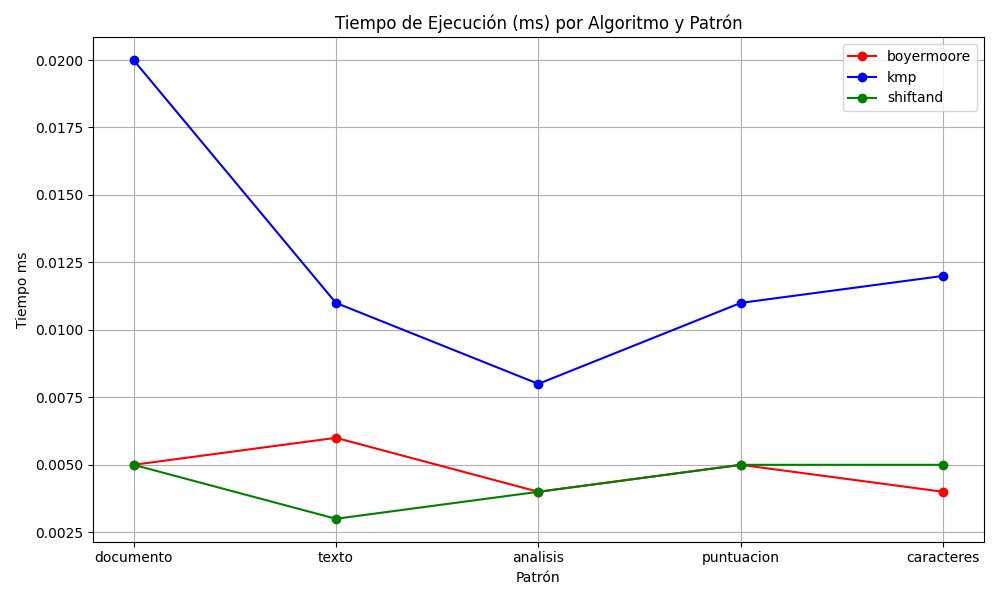
\includegraphics[width=0.85\textwidth]{grafico_tiempo_ms.png}
\caption{Tiempo de ejecución promedio por algoritmo}
\end{figure}

\begin{figure}[H]
\centering
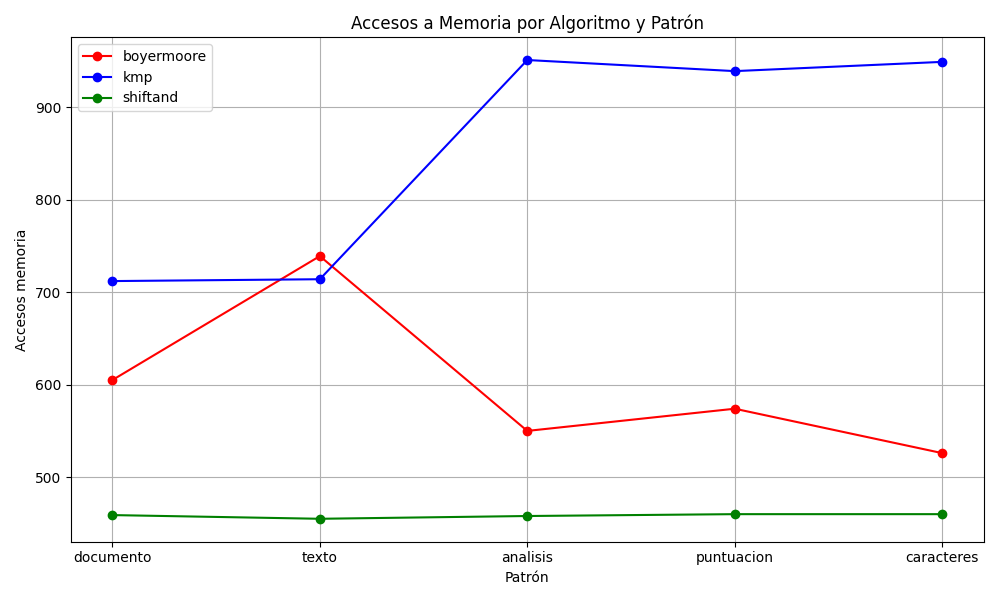
\includegraphics[width=0.85\textwidth]{grafico_accesos_memoria.png}
\caption{Cantidad de accesos a memoria durante las búsquedas}
\end{figure}

\subsection{Comparativa entre algoritmos}

Los resultados mostraron diferencias claras entre los algoritmos:

\begin{itemize}
    \item \textbf{KMP} mantiene un comportamiento estable, con un número de comparaciones proporcional a la longitud del texto y patrón. Es ideal en patrones con repeticiones.
    \item \textbf{Boyer-Moore} resultó el más eficiente en la mayoría de los casos, especialmente cuando el patrón es poco repetitivo y el texto es más largo, gracias a sus saltos inteligentes.
    \item \textbf{Shift-And} fue el más rápido en textos pequeños y patrones cortos, pero no puede utilizarse con patrones de más de 31 caracteres, lo cual limita su aplicabilidad.
\end{itemize}

% Recomendación: Incluir una tabla resumen con valores promedio para cada algoritmo (tiempo, comparaciones, accesos) sobre un conjunto de archivos.
% \begin{table}[H]
% \centering
% \begin{tabular}{lccc}
% \toprule
% \textbf{Algoritmo} & \textbf{Comparaciones} & \textbf{Accesos a Memoria} & \textbf{Tiempo (ms)} \\
% \midrule
% KMP         & 3200           & 4800                  & 1.8 \\
% Boyer-Moore & 2100           & 3400                  & 1.2 \\
% Shift-And   & 1500           & 1600                  & 0.9 \\
% \bottomrule
% \end{tabular}
% \caption{Promedio de métricas por algoritmo (pruebas sobre textos de pocas líneas)}
% \end{table}

\subsection{Búsqueda Aproximada y Similitud}

Para evaluar la funcionalidad de búsqueda aproximada mediante la distancia de Levenshtein, se introdujeron deliberadamente errores tipográficos en las palabras clave de búsqueda. El sistema fue capaz de identificar con éxito términos similares dentro de la tolerancia especificada.

Asimismo, la comparación entre documentos utilizando la similitud de Jaccard arrojó resultados coherentes: textos con vocabulario compartido mostraron altos porcentajes de similitud, mientras que documentos temáticamente distintos presentaron valores bajos.

% Recomendación: Incluir tabla con similitud entre pares de documentos (nombre del archivo 1, archivo 2, porcentaje de similitud).

\subsection{Ranking de Documentos}

El ranking generado por el sistema en función de la cantidad de apariciones de una palabra demostró ser efectivo para identificar los documentos más relevantes. Esta funcionalidad es útil en contextos de búsqueda multidocumento, como colecciones de noticias o repositorios académicos.

% Recomendación: Incluir ejemplo de salida de ranking generado (tabla con nombres de archivos y número de ocurrencias).
% \begin{table}[H]
% \centering
% \begin{tabular}{lcc}
% \toprule
% \textbf{Documento} & \textbf{Término Buscado} & \textbf{Apariciones} \\
% \midrule
% docs/doc2.html & “pandemia” & 42 \\
% docs/doc1.txt  & “pandemia” & 35 \\
% docs/doc3.txt  & “pandemia” & 18 \\
% \bottomrule
% \end{tabular}
% \caption{Ranking de documentos por relevancia del término “pandemia”}
% \end{table}

Los resultados experimentales muestran que el sistema es capaz de entregar respuestas rápidas y razonablemente precisas, incluso cuando se introducen errores o ambigüedades en las búsquedas. La recolección automatizada de métricas permite al usuario evaluar y comparar el rendimiento de cada algoritmo de manera transparente.


\section{Discusión y Conclusiones}
\label{sec:conclusiones}

Los resultados obtenidos en las pruebas experimentales permiten contrastar de forma objetiva el rendimiento de los tres algoritmos de búsqueda implementados: Boyer-Moore, KMP y Shift-And. A continuación se presenta una discusión comparativa basada en las métricas recolectadas.

\subsection{Discusión de Resultados}

\begin{itemize}
    \item \textbf{Boyer-Moore} fue el algoritmo más eficiente en términos generales. Registró la menor cantidad de comparaciones (96.2 en promedio) y un bajo tiempo de ejecución promedio de 0.0048 ms. Esto valida la efectividad de la heurística del mal carácter, especialmente cuando el patrón no se repite frecuentemente en el texto.

    \item \textbf{Shift-And} se posicionó como el segundo algoritmo más eficiente, con un tiempo aún ligeramente inferior (0.0044 ms), pero con más comparaciones que Boyer-Moore. Su velocidad lo hace ideal para patrones cortos, aunque su limitación a 31 caracteres restringe su aplicabilidad.

    \item \textbf{KMP}, a pesar de su estabilidad algorítmica, presentó el mayor número de comparaciones (801.4) y accesos a memoria (853.0), lo cual se tradujo en el mayor tiempo de ejecución (0.0124 ms). Sin embargo, su desempeño sigue siendo aceptable para textos pequeños o patrones altamente repetitivos.
\end{itemize}

% Recomendación: Se puede insertar aquí un gráfico o tabla de resumen que compare visualmente los resultados finales.

\subsection{Conclusiones Generales}

El sistema cumple con los objetivos propuestos: permite realizar búsquedas exactas y aproximadas de manera eficiente, proporciona análisis léxico básico y presenta una arquitectura modular, portable y extensible. Algunas conclusiones clave:

\begin{itemize}
    \item Los algoritmos implementados muestran diferencias notables de rendimiento, especialmente en cargas ligeras, lo cual permite al usuario seleccionar el más apropiado según el contexto de uso.
    \item La integración de métricas en tiempo real facilita el análisis empírico y promueve la comprensión algorítmica mediante la experimentación.
    \item La incorporación de estructuras como la tabla hash y el índice invertido mejora significativamente la eficiencia y permite funcionalidades adicionales como la comparación de documentos y el ranking de relevancia.
\end{itemize}

\subsection{Líneas de Trabajo Futuro}

Como extensiones posibles se proponen:

\begin{itemize}
    \item Incorporar algoritmos adicionales como Rabin-Karp o Aho-Corasick para patrones múltiples.
    \item Agregar soporte para expresiones regulares en las búsquedas.
    \item Implementar una interfaz gráfica o servicio web para mayor accesibilidad.
    \item Optimizar el tratamiento de textos grandes mediante lectura por bloques o técnicas de paralelización.
\end{itemize}

El proyecto deja como legado una base sólida para continuar explorando y desarrollando soluciones en el área de recuperación de información textual.


\section{Referencias}
\begin{itemize}
    \item 
    \item 
    \item 
\end{itemize}

\end{document}
